\documentclass{article}

\usepackage{geometry}
\geometry{margin=2cm}
\usepackage{graphicx}
\usepackage{hyperref}
\usepackage{amsfonts}

\hypersetup{colorlinks=true, linkcolor=blue, urlcolor=blue}
\urlstyle{same}
\begin{document}
	
	\author{Aayush Arya}
	\date{(Submitted: \today)}
	\title{}
	
	\maketitle
	
	\hrule
	\begin{center}
		PHY350 Lab Report\\
		Practical: 5 \quad Registration No.: 11912610 \quad Section: G2903
	\end{center}
	\hrule
	
	\section*{Aim}
	To study the power characteristics of a photoresistor.
	
	\section*{Methods}
	The simulation was performed at \url{http://www.falstad.com/circuit/}. A photoresistor's light exposure was varied at constant battery supply voltage of $5V$
	\begin{figure}[h]
		\centering
		\includegraphics[width=0.6\textwidth]{circuit_falstad}
		\caption{A photoresistor circuit using Falstad's online simulator}
	\end{figure}

	Since at constant voltage, power $$P = VI$$ we expect a straight line between $P$ and $I$. Also, since resistance $R$ affects the current as $I = V/R$, $$ P = \frac{V^2}{R}$$ Therefore, a plot of $P$ vs $R$ should look like a rectangular hyperbola.
	
	\section*{Results \& Discussion}
	We verify the expectations described in the preceding section. Our observations have been summarized in Table \ref{tab:data}.
	\begin{table}[h!]
		\centering
		\begin{tabular}{|c|c|c|}
			\hline
			Resistance & Current (mA) & Power (mW)\\
			\hline
			999 & 5.005 & 25.025\\
			1989 & 2.514 & 12.569\\
			2979 & 1.678 & 8.392\\
			3969 & 1.26 & 6.299\\
			5949 & 0.84 & 4.202\\
			9909 & 0.504 & 2.523\\
			14859 & 0.336 & 1.682\\
			29709 & 0.168 & 0.842\\
			50499 & 0.099 & 0.495\\
			99999 & 0.05 & 0.25\\
			\hline
		\end{tabular}
		\caption{Measurements at constant $V_d = 5$ V}
		\label{tab:data}
	\end{table}

	The data is plotted in the figure below
	
	\begin{figure}[h]
		\centering
		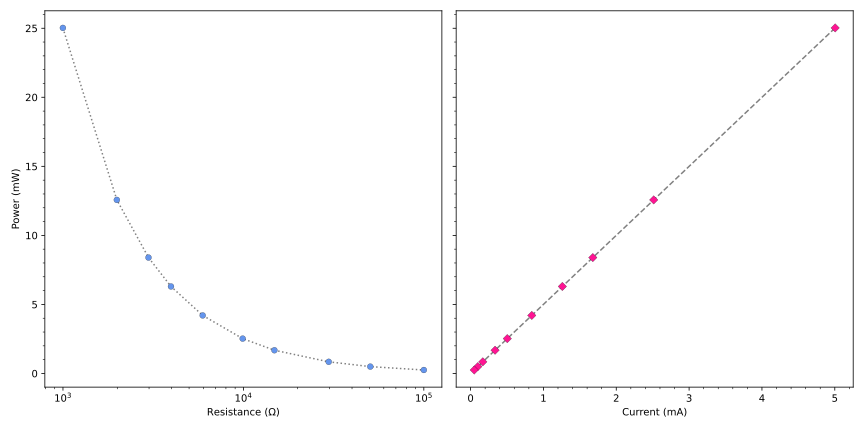
\includegraphics[width=0.9\textwidth]{power_characs}
	\end{figure}

From the plot above, it is evident that $P = VI$ is being strictly followed in a wide range of resistances. Photoresistors thus show the behavior of ohmic resistors and can be considered to be {\it linear} circuit elements.
\end{document}